\section{Results}
\label{sec:results}

\subsection{LiDAR Map Generation using KISS-ICP}

A sample LiDAR scan from the KITTI Odometry dataset and the final map generated from 100 scans from the first sequence is demonstrated in \autoref{fig:lidar_scans}. The alignment by KISS-ICP resulted in a absolute trajectory error of 0.082m and an absolute rotational error of 0.061rad.

\begin{figure*}[t]
    \centering
    \begin{subfigure}[t]{0.49\textwidth}
        \centering
        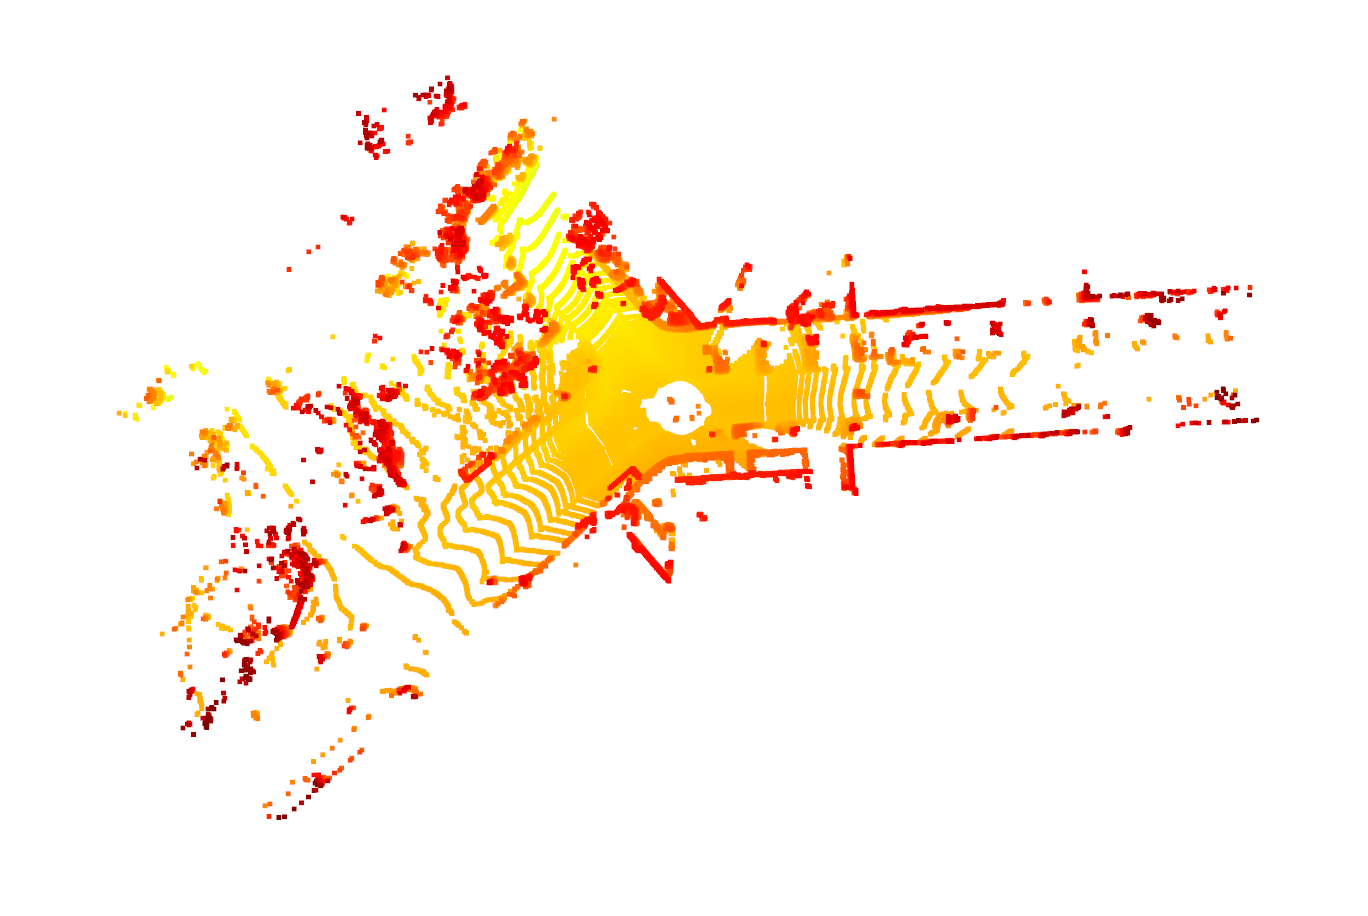
\includegraphics[width=\textwidth]{figures/lidar_frame.png}
        \caption{Sample LiDAR Scan}
    \end{subfigure}
    \begin{subfigure}[t]{0.49\textwidth}
        \centering
        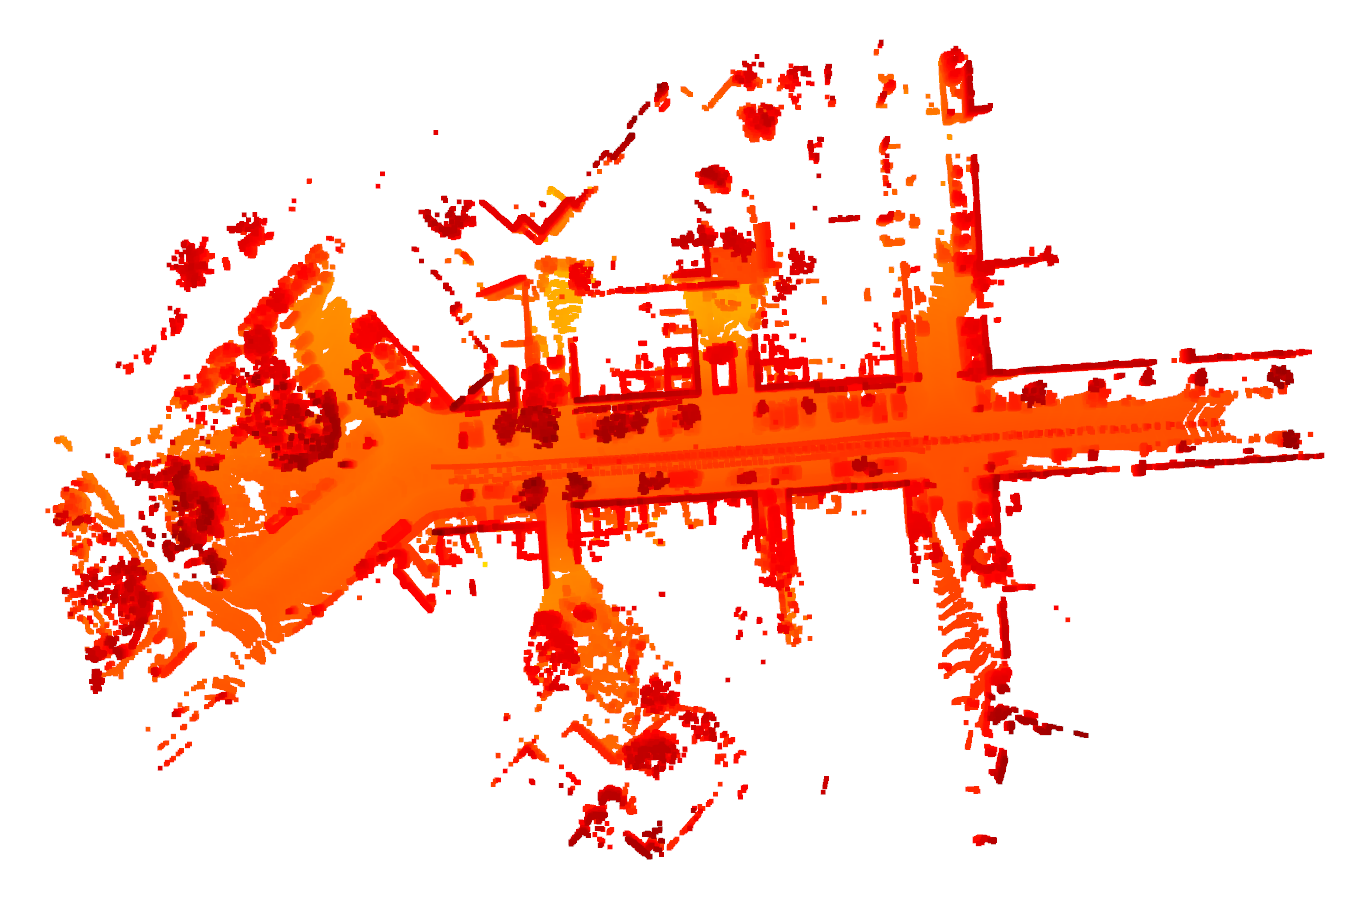
\includegraphics[width=\textwidth]{figures/lidar_map.png}
        \caption{LiDAR Map constructed Using ICP}
    \end{subfigure}
    \caption{Visualization of a sample LiDAR scan and the corresponding LiDAR map constructed using ICP.}
    \label{fig:lidar_scans}
\end{figure*}

\subsection{Ablation Study on 3D-BBS}
The ablation studies reveal the sensitivity of the 3D-BBS algorithm to its configuration parameters, as shown in \autoref{fig:ablation_study}. Increasing \textit{max\_scan\_range}, \textit{min\_level\_res}, and decreasing \textit{src\_leaf\_size} enhances localization accuracy by enabling finer pose subdivisions, reducing translation errors effectively. However, this comes with a trade-off in processing time, as the number of candidate poses increases exponentially with each additional hierarchical level. We did not find any significant pattern with other parameters.

\begin{figure*}[t]
    \centering
    \begin{subfigure}[t]{0.32\textwidth}
        \centering
        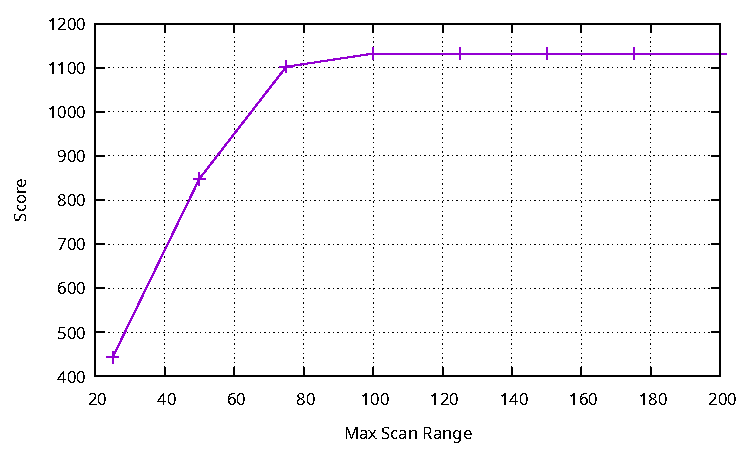
\includegraphics[width=\textwidth]{../02-global-localization/plots/max_scan_range.pdf}
        \caption{Max Scan Range}
    \end{subfigure}
    \begin{subfigure}[t]{0.32\textwidth}
        \centering
        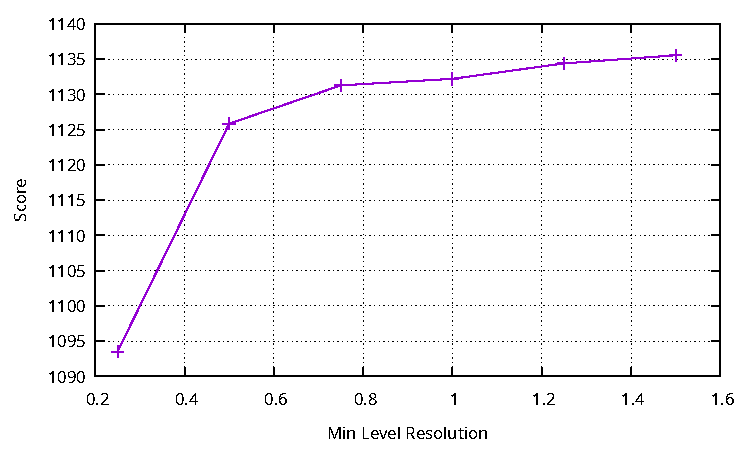
\includegraphics[width=\textwidth]{../02-global-localization/plots/min_level_res.pdf}
        \caption{Min Level Resolution}
    \end{subfigure}
    \begin{subfigure}[t]{0.32\textwidth}
        \centering
        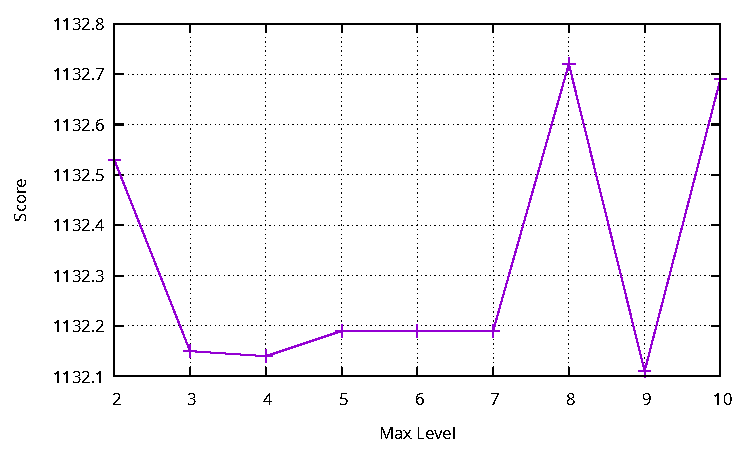
\includegraphics[width=\textwidth]{../02-global-localization/plots/max_level.pdf}
        \caption{Max Level}
    \end{subfigure}
    \begin{subfigure}[t]{0.32\textwidth}
        \centering
        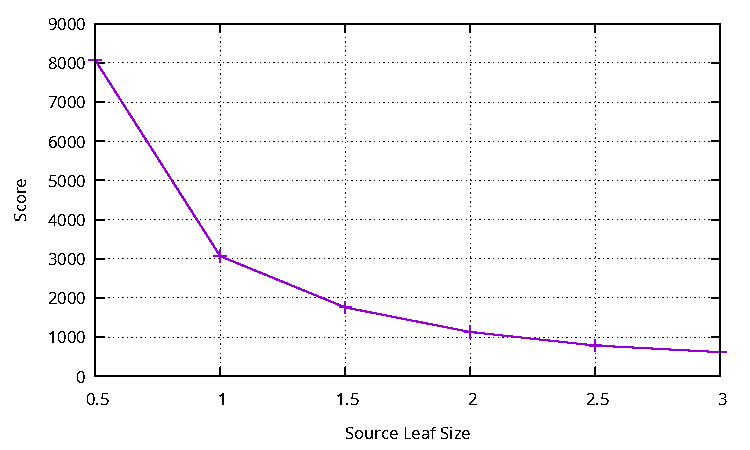
\includegraphics[width=\textwidth]{../02-global-localization/plots/src_leaf_size.pdf}
        \caption{Source Leaf Size}
    \end{subfigure}
    \begin{subfigure}[t]{0.32\textwidth}
        \centering
        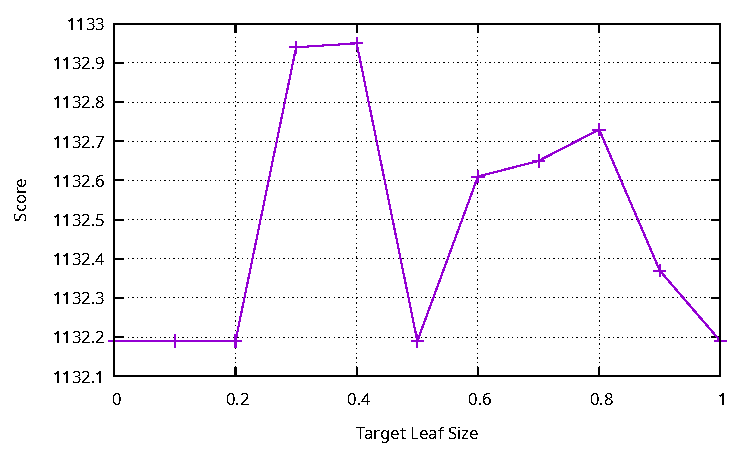
\includegraphics[width=\textwidth]{../02-global-localization/plots/tar_leaf_size.pdf}
        \caption{Target Leaf Size}
    \end{subfigure}
    \caption{Ablation study figures showing change in 3D-BBS localization score with variation in parameters.}
    \label{fig:ablation_study}
\end{figure*}

\subsection{Integration with RGB Images}

A sample RGB image frame from the KITTI Odometry dataset, and the metric depth estimated by Depth Anything v2 is demonstrated in \autoref{fig:image_to_3d_projection}. Note that estimation of metric depth is essential for compatibility of point clouds between different images. We then follow the same procedure with the LiDAR scans to generate a LiDAR map. The resultant map is however not of a very good quality, despite measures such as norm clipping to remove poor estimates of far away points.

\begin{figure*}[t]
    \centering
    \begin{subfigure}[t]{0.49\textwidth}
        \centering
        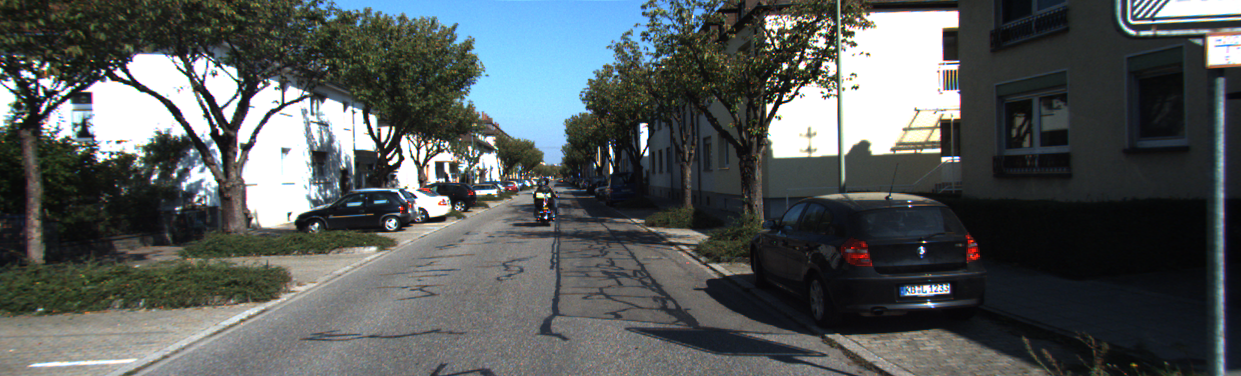
\includegraphics[width=\textwidth]{figures/rgb_image.png}
        \caption{Sample RGB Image}
    \end{subfigure}
    \begin{subfigure}[t]{0.49\textwidth}
        \centering
        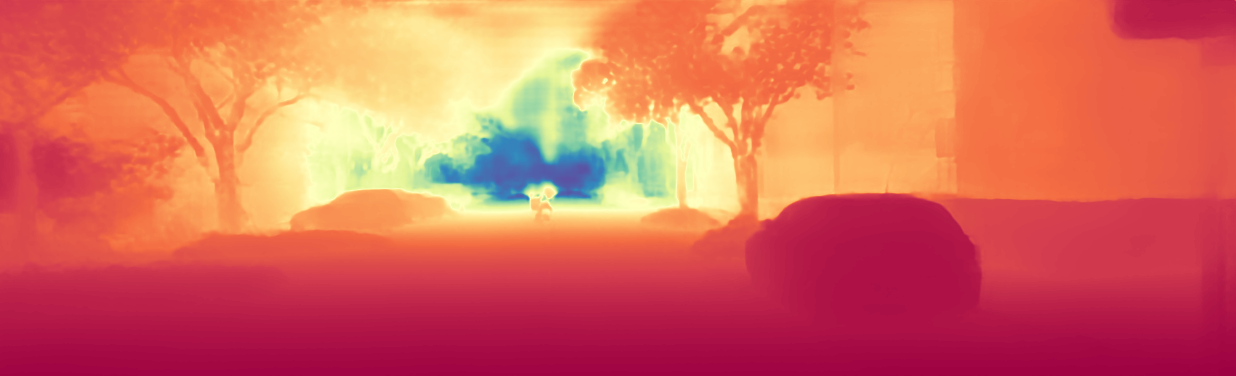
\includegraphics[width=\textwidth]{figures/depth_estimate.png}
        \caption{Metric Depth Estimate}
    \end{subfigure}
    \begin{subfigure}[t]{0.49\textwidth}
        \centering
        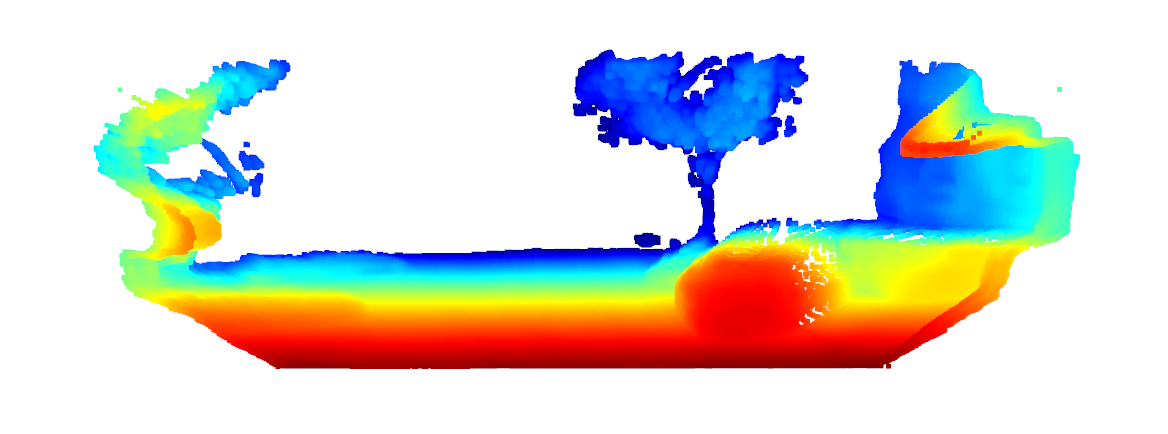
\includegraphics[width=\textwidth]{figures/projected_point_cloud.png}
        \caption{Projected Point Cloud}
    \end{subfigure}
    \begin{subfigure}[t]{0.49\textwidth}
        \centering
        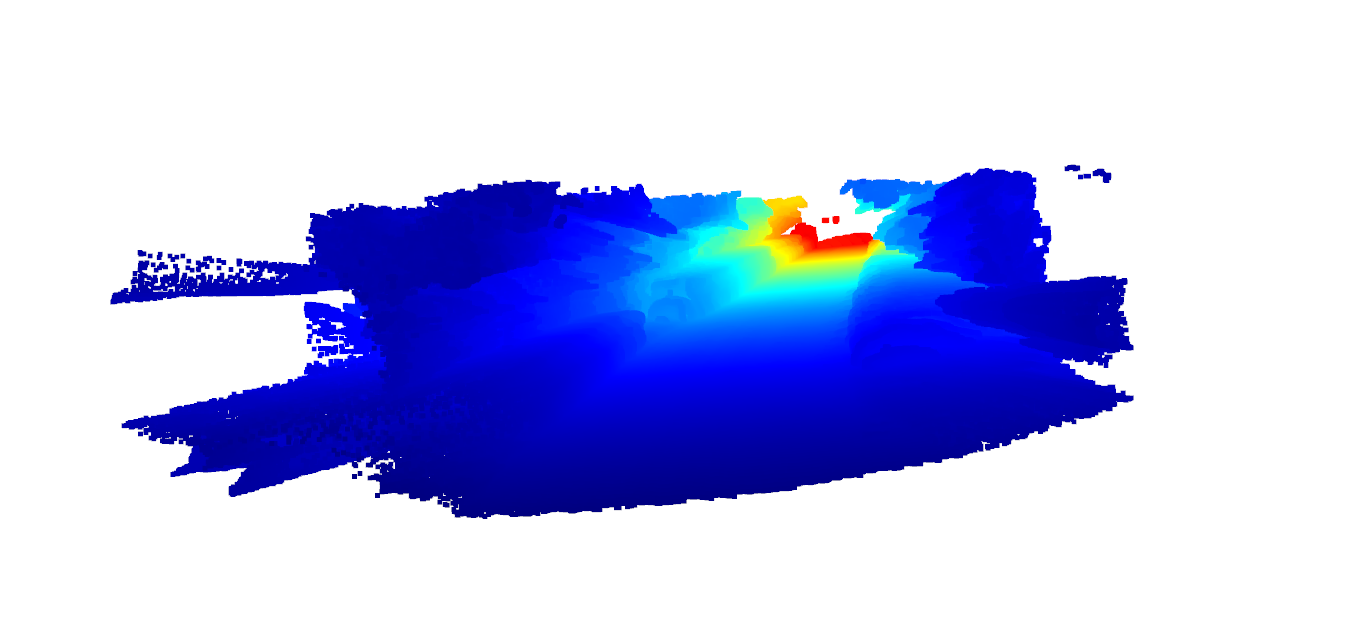
\includegraphics[width=\textwidth]{figures/concatenated_point_cloud.png}
        \caption{Concatenated Point Cloud}
    \end{subfigure}
    \caption{Generation of point cloud by reprojection from the image to 3D space, using depth estimatation.}
    \label{fig:image_to_3d_projection}
\end{figure*}

\subsection{Discussion on 3D-BBS}
The experimental results affirm the efficacy of the 3D-BBS algorithm in achieving accurate and efficient global localization using LiDAR data. The hierarchical BnB approach, combined with sparse voxel mapping and GPU acceleration, addresses the primary challenges associated with 3D localization, including large search spaces and high computational demands.

\subsubsection{Advantages of 3D-BBS}
\begin{itemize}
    \item \textbf{Scalability}: The hierarchical voxel map and sparse representation allow 3D-BBS to scale effectively to large environments without excessive memory consumption.
    \item \textbf{Real-Time Performance}: GPU-accelerated batched processing ensures that localization can be performed within acceptable time frames, making it suitable for real-time applications in autonomous systems.
    \item \textbf{Robustness}: The algorithm maintains high localization accuracy across diverse and dynamic environments, demonstrating resilience against environmental variations and outliers.
    \item \textbf{Flexibility}: The parameter ablation studies provide insights into tuning the algorithm for different scenarios, allowing adaptability to various application requirements.
\end{itemize}

\subsubsection{Limitations and Future Work}
Despite its advantages, the 3D-BBS algorithm has certain limitations that warrant further investigation:

\begin{itemize}
    \item \textbf{Preprocessing Overhead}: The initial voxel map construction is computationally intensive, although it is a one-time cost. Future work could explore incremental map updates to accommodate dynamic environments.
    \item \textbf{Integration with Additional Sensors}: While the integration of RGB images enhances localization, incorporating other sensors such as IMUs or cameras could further improve robustness and accuracy.
    \item \textbf{Adaptive Parameter Tuning}: Developing adaptive mechanisms for parameter tuning based on environmental conditions could enhance the algorithm's flexibility and performance across varied scenarios.
    \item \textbf{Handling Extreme Cases}: Extending the algorithm to handle extreme cases, such as degenerated areas with minimal features or significant occlusions, remains an area for future research.
\end{itemize}

